% --------------------------------------------------------------
% This is all preamble stuff that you don't have to worry about.
% Head down to where it says "Start here"
% --------------------------------------------------------------
 
\documentclass[11pt]{article}
 
\usepackage[margin=0.6in]{geometry} 
\usepackage{amsmath,amsthm,amssymb,mathtools}
\usepackage{enumerate} 
\usepackage{graphicx,float} % figures
\usepackage{csvsimple,longtable,booktabs} % load csv as a table
\usepackage{listings,color} % for code snippets


%%======%%
% All this is to force LaTeX to prefix "Appendix" before a new appendix section letter
\makeatletter
% The "\@seccntformat" command is an auxiliary command
% (see pp. 26f. of 'The LaTeX Companion,' 2nd. ed.)
\def\@seccntformat#1{\@ifundefined{#1@cntformat}%
   {\csname the#1\endcsname\quad}  % default
   {\csname #1@cntformat\endcsname}% enable individual control
}
\let\oldappendix\appendix %% save current definition of \appendix
\renewcommand\appendix{%
    \oldappendix
    \newcommand{\section@cntformat}{\appendixname~\thesection\quad}
}
\makeatother
%%======%%

%%======%%
% Define for code section
\definecolor{dkgreen}{rgb}{0,0.6,0}
\definecolor{gray}{rgb}{0.5,0.5,0.5}
\definecolor{mauve}{rgb}{0.58,0,0.82}

\lstset{frame=tb,
  language=C++,
  aboveskip=3mm,
  belowskip=3mm,
  showstringspaces=false,
  columns=flexible,
  basicstyle={\scriptsize\ttfamily},
  numbers=none,
  numberstyle=\tiny\color{gray},
  keywordstyle=\color{blue},
  commentstyle=\color{dkgreen},
  stringstyle=\color{mauve},
  breaklines=true,
  breakatwhitespace=true,
  tabsize=3
}
%%======%%
%% set noindent by default and define indent to be the standard indent length
\newlength\tindent
\setlength{\tindent}{\parindent}
\setlength{\parindent}{0pt}
\renewcommand{\indent}{\hspace*{\tindent}}

\begin{document}
 
% --------------------------------------------------------------
%                         Start here
% --------------------------------------------------------------
 
\title{Assignment 3}
\author{David Fleischer\\ 
MACF 402 - Mathematical \& Computational Finance II}
 
\maketitle
\section{Question 1: {\normalfont Programming a Black-Scholes Implied Volatility Calculator}}

\subsection{Numerical Solutions to the Normal CDF}

We first investigate our (naive) numerical approximation to the standard normal CDF
\begin{equation*}
	\Phi(x) \approx 1 - \phi(x)(b_1 t + b_2 t^2 + b_3 t^3 + b_4 t^4 + b_5 t^5)
\end{equation*}

where $b_0 = 0.2316419, b_1 = 0.319381530, b_2 = -0.356563782, b_3 = 1.781477937$, $b_4 = -1.821255978, b_5 = 1.330274429$, and $t = \frac{1}{1 + b_0x}$. \\

\indent Comparing our approximation to the true value of the normal CDF (as computed by R's \texttt{pnorm}) we see that the approximation is reasonable for positive values of $x$ but is a failure for $x$ negative. In particular, Figure \ref{fig:naive_approx1} shows that values of the normal CDF approximation for $x \in [-3,3]$ and $x \in [-4,-3]$ are not usable for $x$ negative, becoming an increasingly poor approximation as $x$ decreases. We also notice a nasty singularity present itself in our approximation when $1 + b_0x = 0 \iff x = \frac{-1}{0.2316419} \approx -4.317$. Figure \ref{fig:naive_approx_error} completes the point, showing us that the error between the true value of the normal CDF and our approximation is acceptable for only $x > 0$.

\begin{figure}[H]
	\centering
 	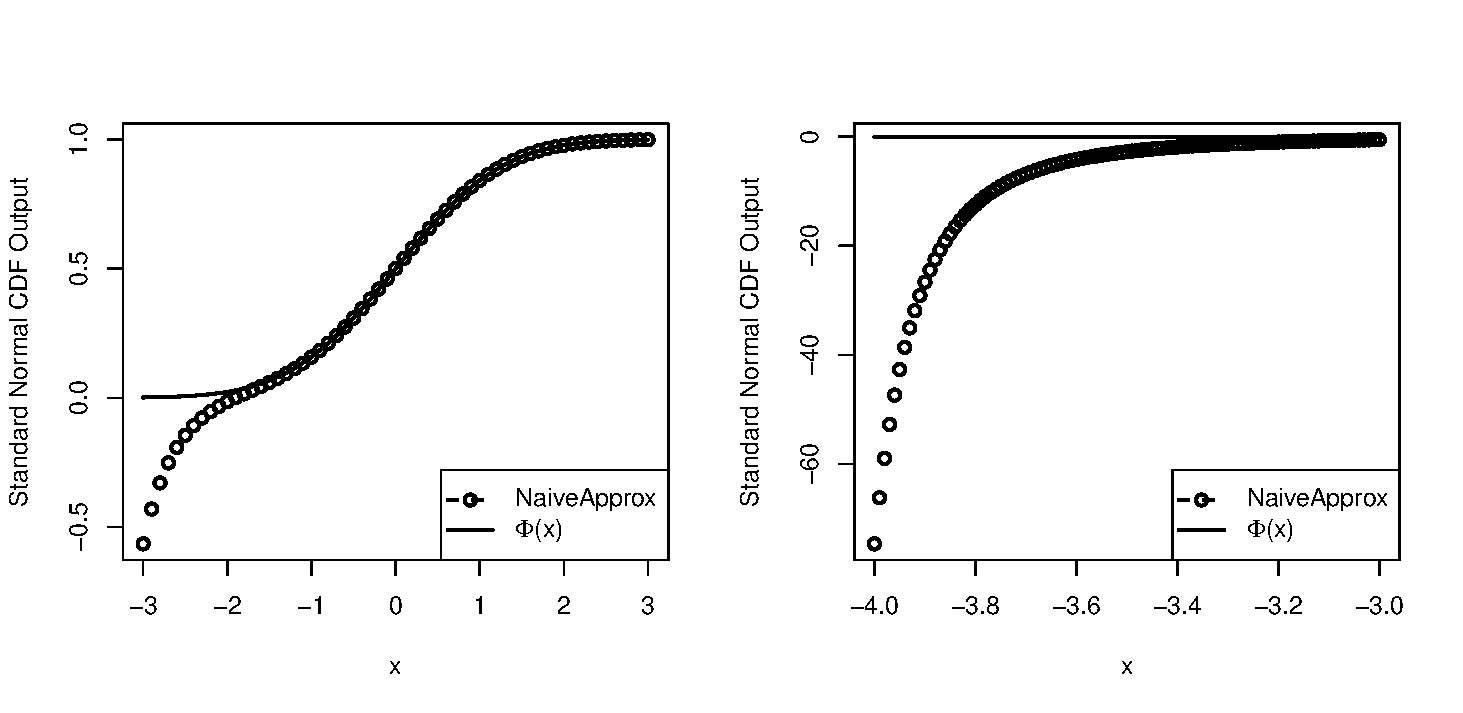
\includegraphics[scale=0.55]{../plots/q1/naive_approx1.pdf}
\caption{(Left) The approximation to the normal CDF described above is successful for positive $x$ but for negative $x$ is a poor approximation. (Right) Increasingly negative values of $x$ show completely unusable approximations of the normal CDF.}
\label{fig:naive_approx1}
\end{figure}

\begin{figure}[H]
	\centering
 	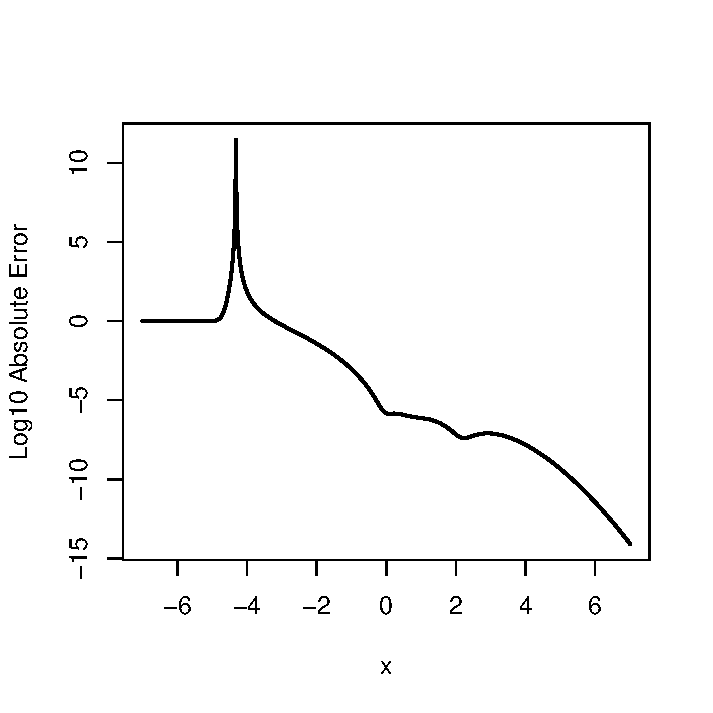
\includegraphics[scale=0.55]{../plots/q1/naive_approx_error.pdf}
\caption{The error between the normal approximation and the true value of the normal CDF is sufficiently small for $x$ large but for $x$ small the error is too large to be usable. For $x$ small the value of the error settles to $\approx 10^0 = 1$: Completely unusable as a CDF.}
\label{fig:naive_approx_error}
\end{figure}

\indent To solve this problem we note that our function is suitable for $x$ positive and rely on the symmetry of the normal distribution. In particular, we use
\begin{equation*}
	\Phi(-x) = 1 - \Phi(x)
\end{equation*}

From this, we find our new approximation to the normal CDF
\begin{equation*}
	\Phi(x) \approx
	\begin{cases}
		1 - \phi(x)(b_1 t(x) + b_2 [t(x)]^2 + b_3 [t(x)]^3 + b_4 [t(x)]^4 + b_5 [t(x)]^5) & x \geq 0 \\
		\phi(-x)(b_1 t(-x) + b_2 [t(-x)]^2 + b_3 [t(-x)]^3 + b_4 [t(-x)]^4 + b_5 [t(-x)]^5) & x < 0
	\end{cases}
\end{equation*}

\indent Figure \ref{fig:lessnaive_approx_error} shows us that this new implementation is a significant improvement to our earlier attempt. With the normal approximation complete we move on to other issues.

\begin{figure}[H]
	\centering
 	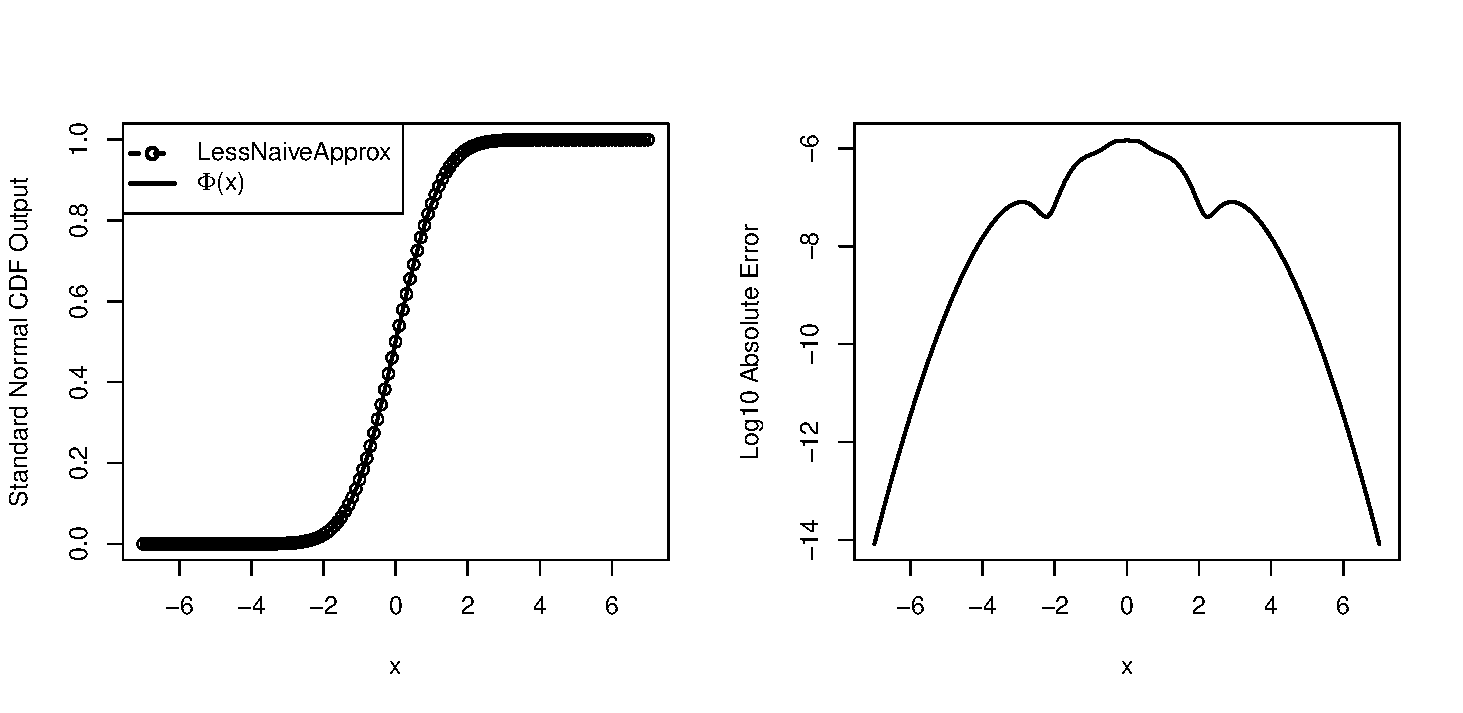
\includegraphics[scale=0.55]{../plots/q1/lessnaive_approx_error.pdf}
\caption{(Left) The new implementation of the normal approximation is appreciably more accurate than the implementation first introduced. (Right) The absolute error for all $x$ is now sufficiently small (for our purposes).}
\label{fig:lessnaive_approx_error}
\end{figure}

\subsection{Computing Implied Volatilities}

\indent We now use our closed form expression (approximation) for the normal CDF to compute the Black-Scholes price of a European. That is, we have
\begin{align*}
	C(S,K, t, T, r, \sigma) &= \Phi(d_1)S - \Phi(d_2)Ke^{-r(T - t)} \\
	P(S,K, t, T, r, \sigma) &= \Phi(-d_2)Ke^{-r(T - t)} - \Phi(-d_1)S
\end{align*}

with 
\begin{align*}
	d_1 &= \frac{1}{\sigma\sqrt{T - t}} \bigg[\ln\bigg(\frac{S}{K}\bigg) + \bigg(r + \frac{\sigma^2}{2}\bigg)(T - t) \bigg]\\
	d_2 &= d_1 - \sigma\sqrt{T - t}
\end{align*}

and option Delta \& Vega\footnote{Derivations of option Delta and Vega are presented in an appendix.}
\begin{align*}
	\Delta_C &= \Phi(d_1) \\
	\Delta_P &= -\Phi(-d_1) \\
	\nu_C = \nu_P &= S\phi(d_1)\sigma\sqrt{T - t}
\end{align*}

\indent With our ingredients in place we are now in a position to numerically solve for the Black-Scholes implied volatility for options written on an underlying asset with $S_0 = 4.75, r = 0.0492$ and $\tau = 59/365$ years to maturity.

\begin{figure}[H]
	\centering
 	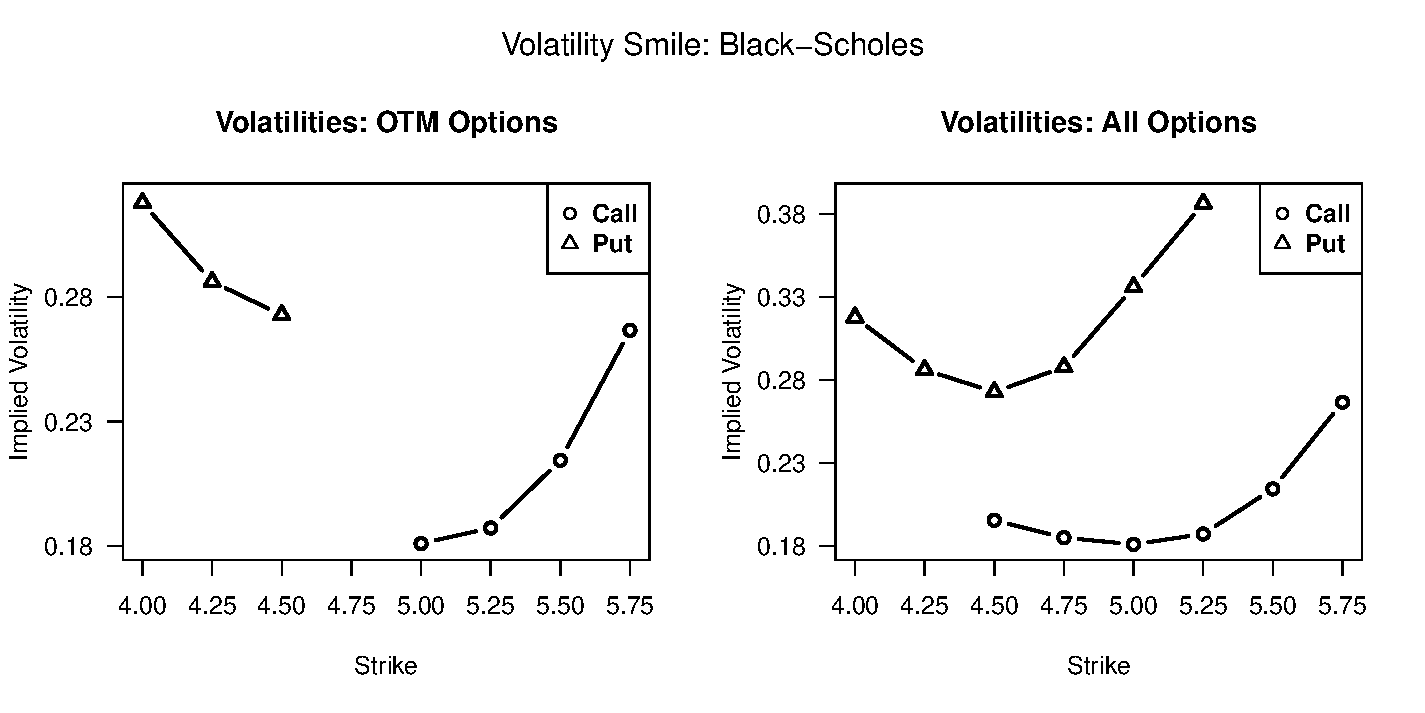
\includegraphics[scale=0.6]{../plots/q1/smile.pdf}
	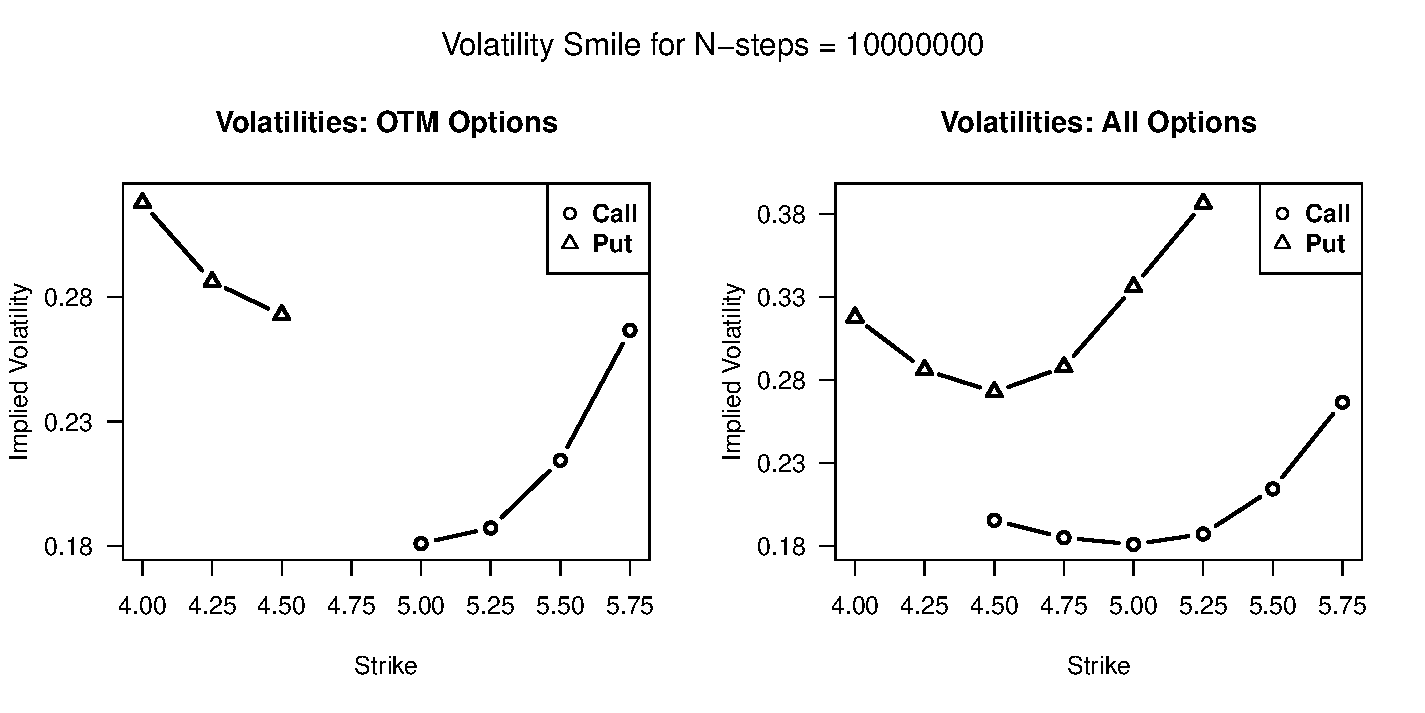
\includegraphics[scale=0.6]{../plots/q1/smile_bin.pdf}
\caption{The volatility smile as computed by the Black-Scholes model (top) and the Binomail model (bottom) for the given asset using only OTM observed option prices (left) and all option prices (right).}
\label{fig:vol_smile}
\end{figure}

\indent Figure \ref{fig:vol_smile} shows us a notable smile, with a discontinuity at $K = S$, when computing the implied volatility with only OTM options. Notably, the Black-Scholes implementation produces implied volatility estimates that are (at least impressionistically) nearly identical to those calculated using the Binomial model. Yielding the same output, the Black-Scholes model is preferable since it is sufficiently closed-form and thus extremely fast. This is a point of comparison with the iterative solution for the Binomial model, which is comparatively slow.

\section{Question 2: {\normalfont Fitting an Implied Volatility Surface}}

\indent For Apple (AAPL) stock on February 17, 2012 with spot price $\$502.12$ we have computed the implied volatility curve for options expiring on March 17, 2012; April 17, 2012; and May 17, 2012, seen in Figure \ref{fig:aapl_smile}. Note that we see a decided volatility smile, as computed by OTM options written on AAPL, in all three maturities.

\begin{figure}[H]
	\centering
 	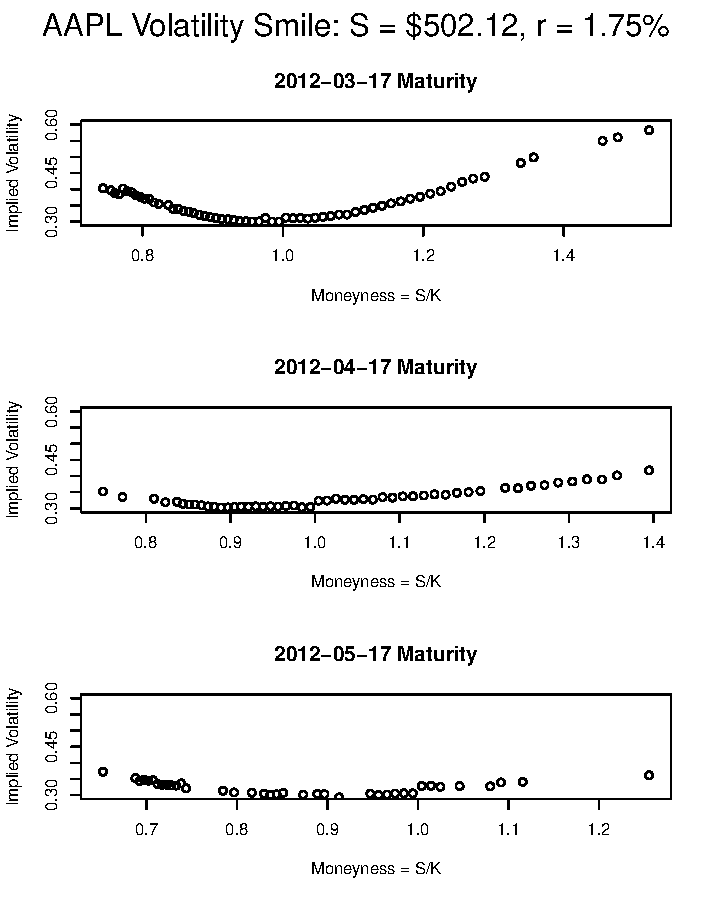
\includegraphics[scale=0.85]{../plots/q2/aapl_smile.pdf}
\caption{The implied volatility curve for AAPL as computed by OTM options. We note the clear volatility smile.}
\label{fig:aapl_smile}
\end{figure}

\subsection{One Dimensional Fitted Estimates}

\indent In order to determine an effective smoothing parameter $h$ for the one dimensional Nadaraya-Watson estimator we perform a bit of exploration in a region of plausible parameters. Plotted in Figures \ref{fig:expl_fitted_mar}, \ref{fig:expl_fitted_apr}, and \ref{fig:expl_fitted_may} are the fitted smiles for March, April, and May maturities, using $h \in \{0.025, 0.05, 0.075, 0.1\}$. Pathological cases for $h$ extremely small/large are considered in the two dimensional estimator.

\begin{figure}[H]
	\centering
 	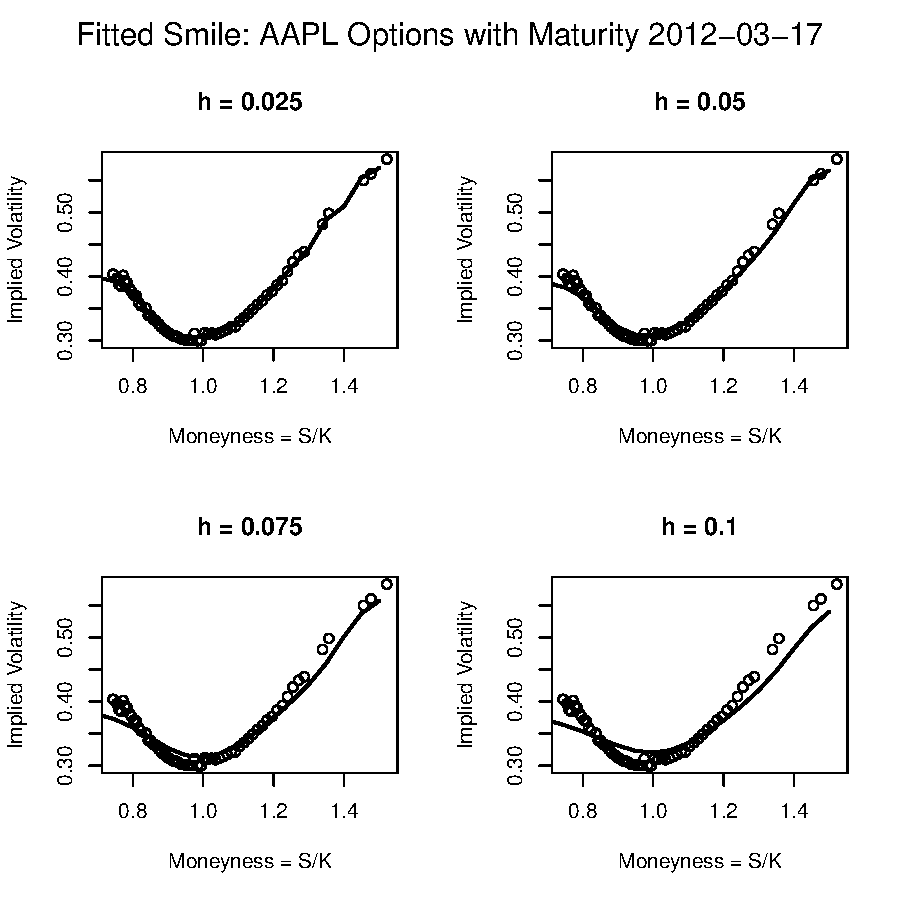
\includegraphics{../plots/q2/expl_fitted_smile_mar.pdf}
\caption{Fitted smiles for options written on AAPL expiring March 17, 2012.}
\label{fig:expl_fitted_mar}
\end{figure}
\begin{figure}[H]
	\centering
 	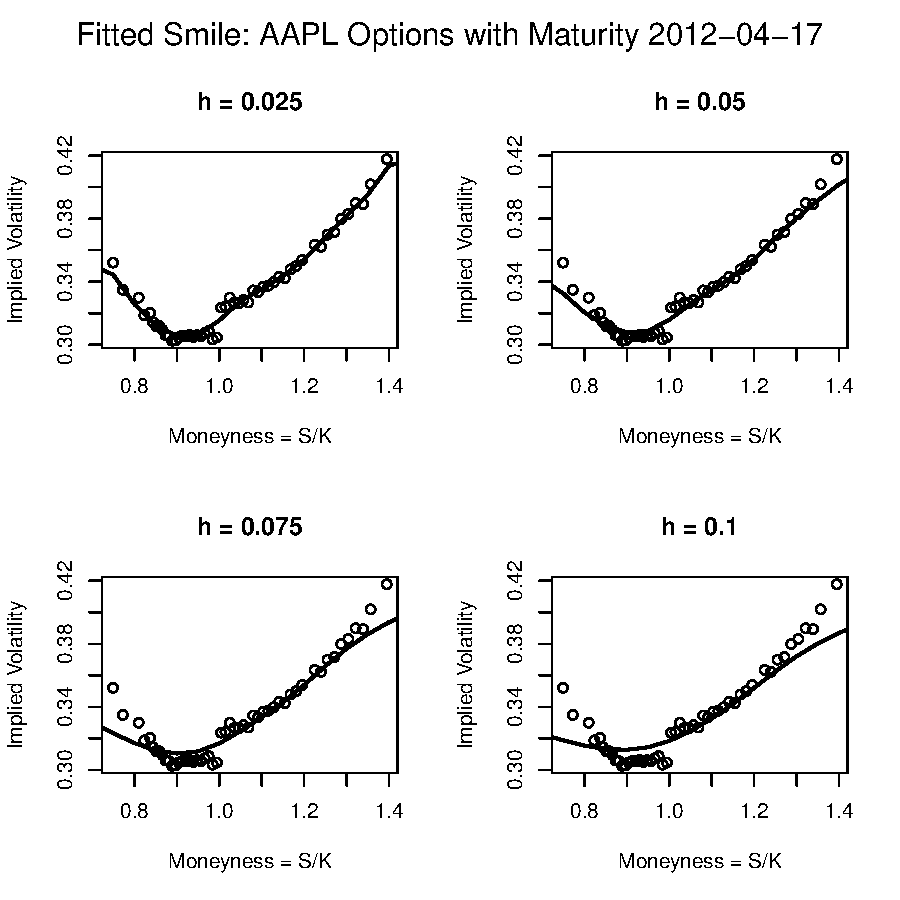
\includegraphics{../plots/q2/expl_fitted_smile_apr.pdf}
\caption{Fitted smiles for options written on AAPL expiring on April 17, 2012.}
\label{fig:expl_fitted_apr}
\end{figure}
\begin{figure}[H]
	\centering
 	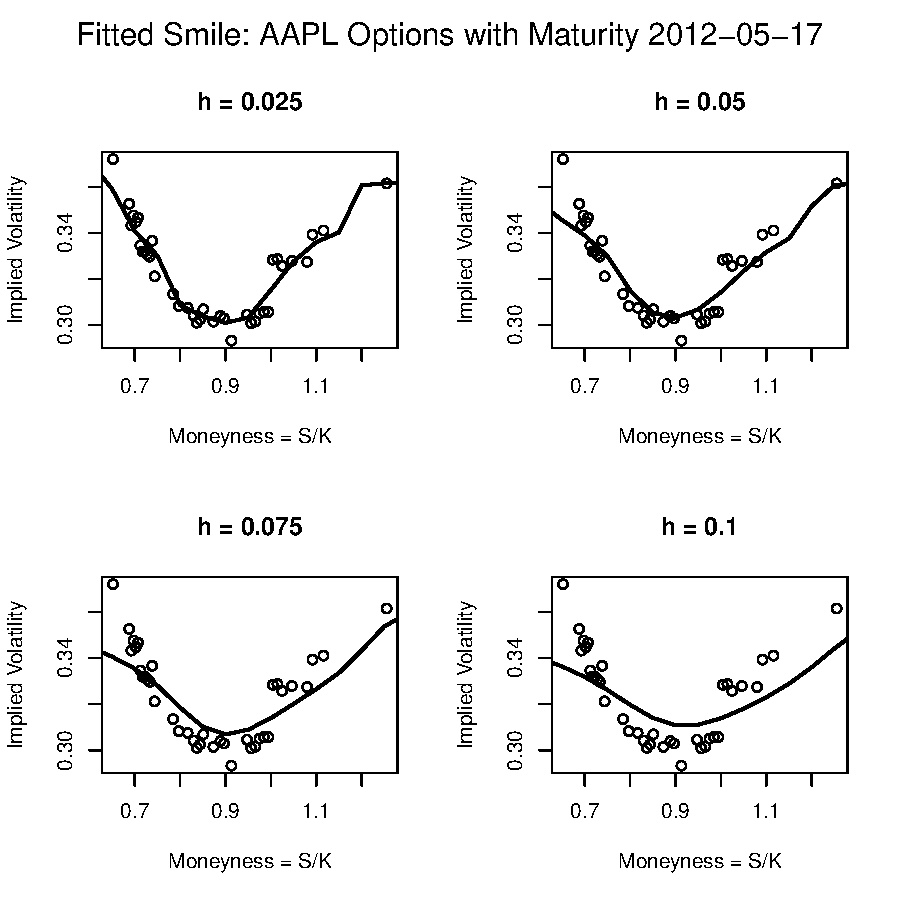
\includegraphics{../plots/q2/expl_fitted_smile_may.pdf}
\caption{Fitted smiles for options written on AAPL expiring on May 17, 2012.}
\label{fig:expl_fitted_may}
\end{figure}

\indent We see that using $h = 0.025$ leads to overfit curves for all maturities, causing several apparent discontinuities. Using $h = 0.05$ provides a reasonably smooth curve for March and April maturities (with the possible exception of extremely high moneyness options for these dates) but leads to overfitting for options expiring in May. Using $h = 0.075$ leads to smooth curves for all maturities, and so we consider $h = 0.075$ as our relatively estimate for $h$ after these trials.

\subsection{Two Dimensional Fitted Estimates}

\subsubsection{Exploration for an Optimal $h_1$, $h_2$}

\indent As the min/max of the domain for the two dimensional Nadayara-Watson estimator we use $(m,t) \in [m_{min}, m_{max}]\times[T_{min},T_{max}] = [0.5,1.5]\times[7/365,105/365]$. We show in Figures \ref{fig:fitted_2d_01_01_0075_0075} and \ref{fig:fitted_2d_005_005} some examples of the volatility surface for different values of $h_1, h_2$. Some pathological cases of overfit/underfit surfaces are provided in an Appendix below. We in Figure \ref{fig:fitted_2d_01_01_0075_0075} that using $h_1 = h_2 = 0.075$ leads to a smooth fitted surface that captures a reasonable amount of detail. Using $h_1 = h_2 = 0.05$ leads to a possibly overfit surface, due to its ``bumpy'' surface features, and so we instead prefer the surface with $h_1 = 0.075, h_2 = 0.075$.

\begin{figure}[H]
	\centering
 	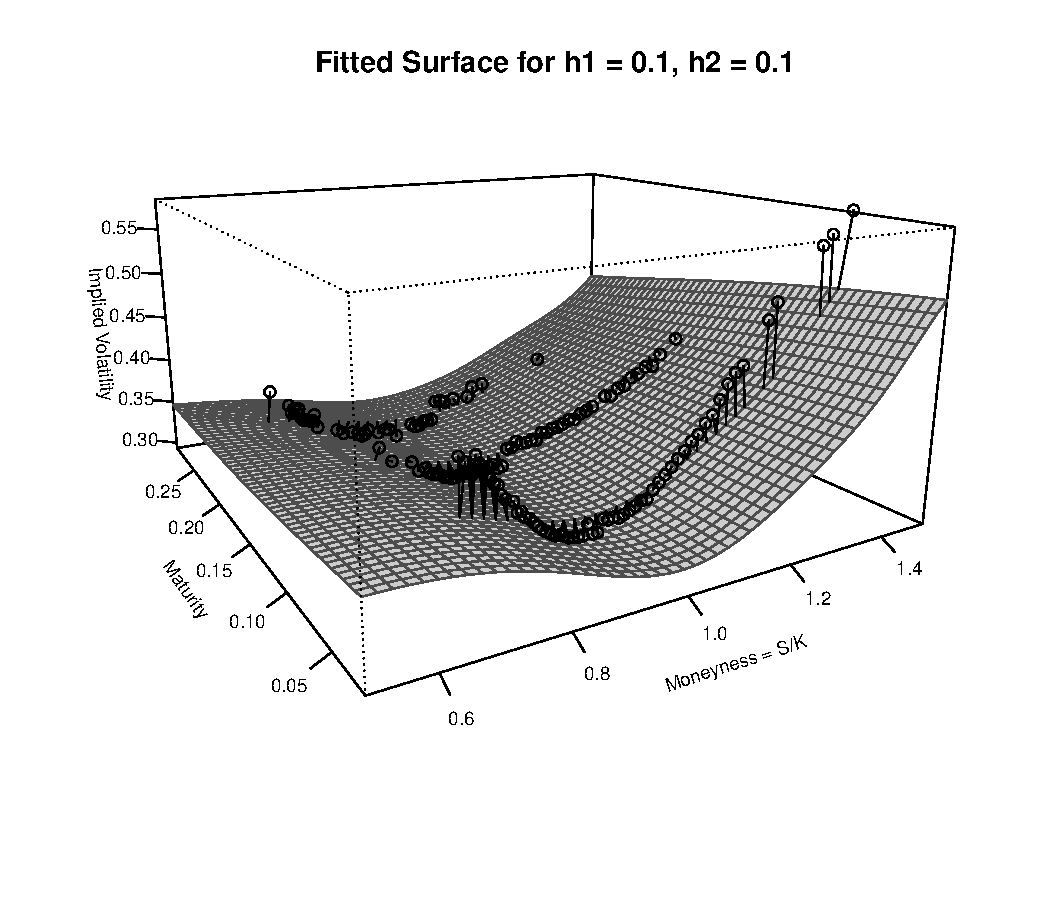
\includegraphics[scale=0.75]{../plots/q2/fitted_2d_01_01.pdf}
	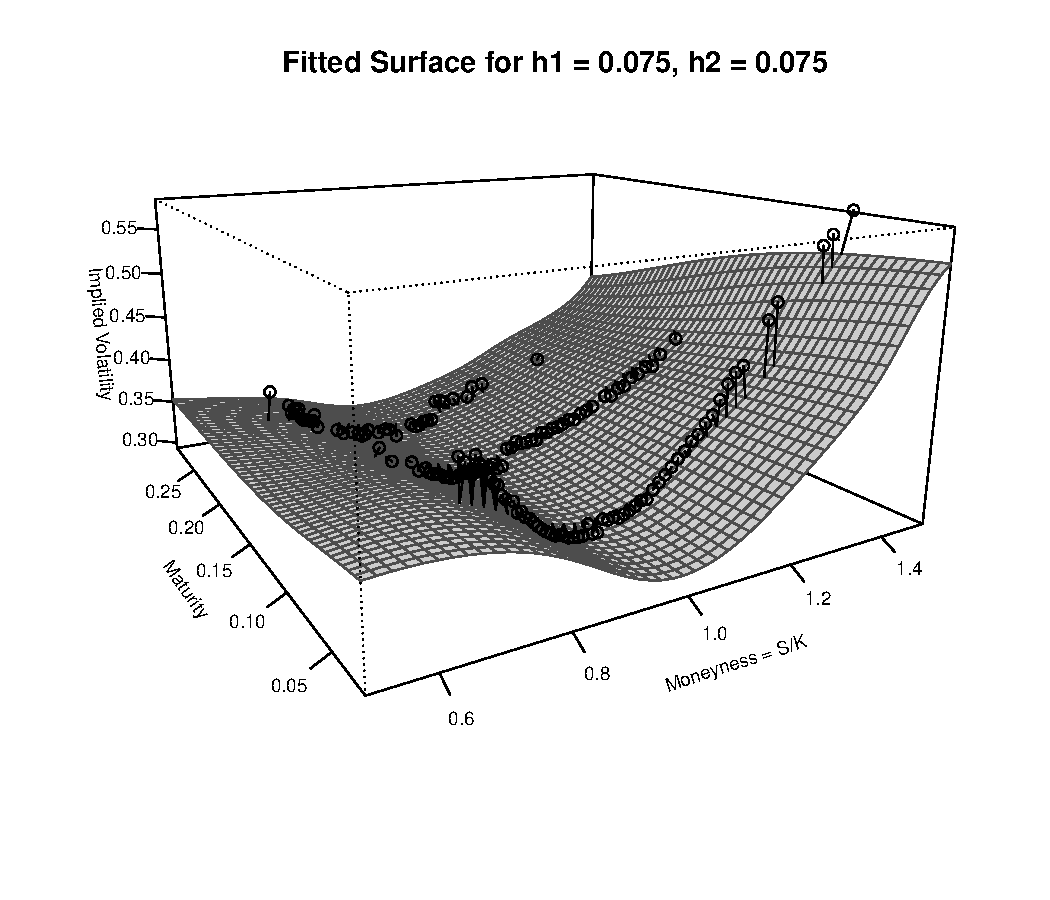
\includegraphics[scale=0.75]{../plots/q2/fitted_2d_0075_0075.pdf}
\caption{Fitted volatility surface for (top) $h_1 = 0.1, h_2 = 0.1$ and (bottom) $h_1 = 0.075, h_2 = 0.075$.}
\label{fig:fitted_2d_01_01_0075_0075}
\end{figure}

\begin{figure}[H]
	\centering
 	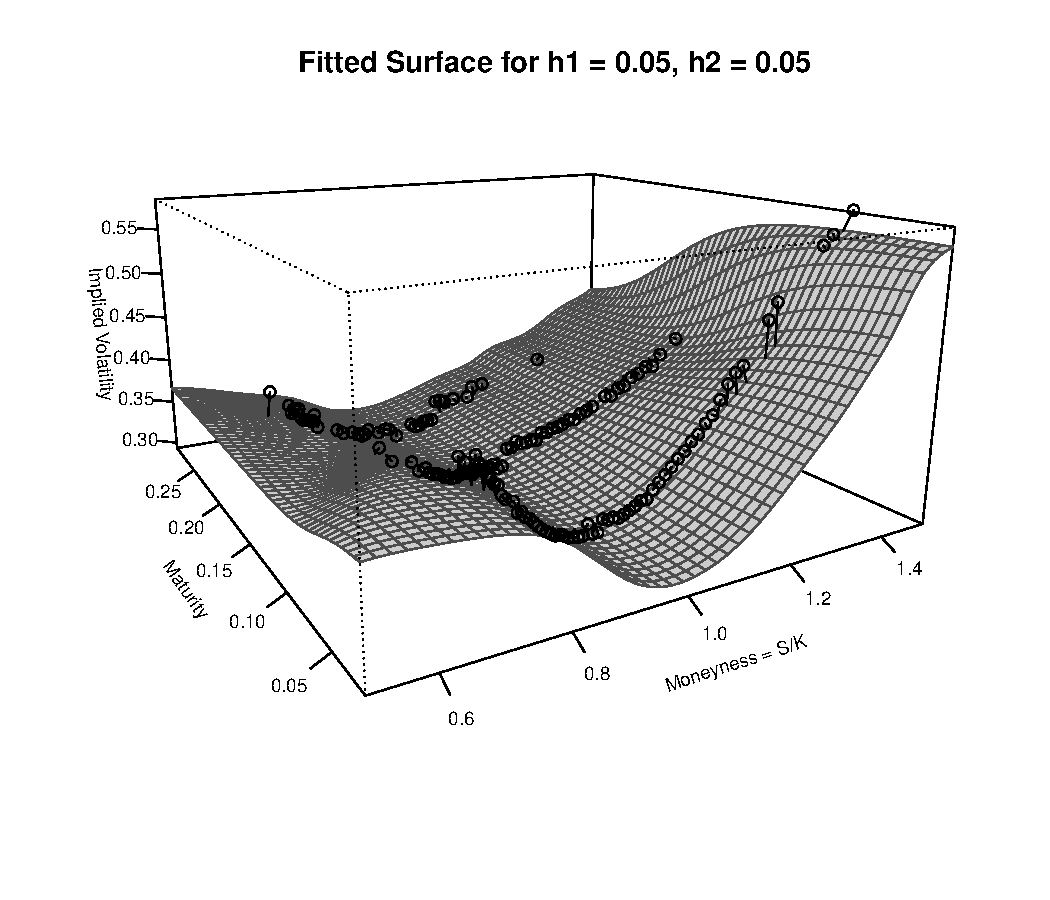
\includegraphics[scale=0.75]{../plots/q2/fitted_2d_005_005.pdf}
\caption{Fitted volatility surface for $h_1 = 0.05, h_2 = 0.05$.}
\label{fig:fitted_2d_005_005}
\end{figure}

\indent Contracting the domain of the Nadaraya-Watson estimator to the min/max of the observed data, we see an appreciable improvement to the fitted volatility surface. Figure \ref{fig:fitted_2d_new_grid} shows us this improved fit by reducing the domain to $(m,t) \in [m_{min}, m_{max}]\times[T_{min},T_{max}] = [502.12/770, 502.12/330]\times[29/365,90/365]$. The observed data appears closer to the volatility surface while still avoiding undue ``bumpiness'' in the surface. In addition, we are able to get away with smaller smoothing parameters $h_1 = h_2 = 0.05$. \\

\indent Reflecting on these results we may conclude that is likely not a very good idea to extrapolate far beyond the observed data. This makes intuitive sense since the Nadayara-Waton Estimator uses observations within the entire range to weight the estimate at a particular point. If we extrapolate beyond the min/max then we are forced to weight the estimate using only data prior to these points, since have no observations beyond these extrema to complete the weighting.

\begin{figure}[H]
	\centering
 	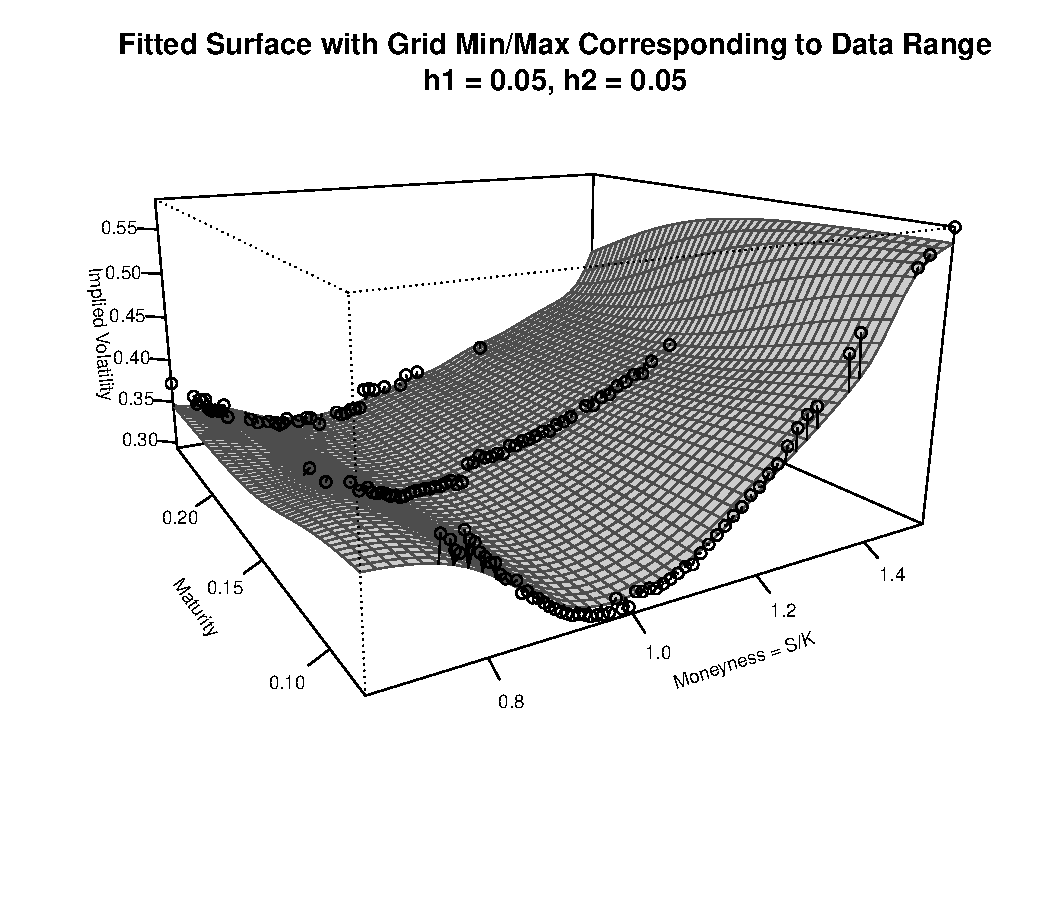
\includegraphics[scale=0.75]{../plots/q2/fitted_2d_new_grid.pdf}
\caption{Fitted volatility surface under the new domain $[m_{min}, m_{max}]\times[T_{min},T_{max}] = [502.12/770, 502.12/330]\times[29/365,90/365]$, with $h_1 = 0.05, h_2 = 0.05$.}
\label{fig:fitted_2d_new_grid}
\end{figure}

\section{Question 3: {\normalfont No Arbitrage Restriction on the Volatility Surfaces}}

For brevity we consider $t = 0$, thus letting $T$ be the time to maturity of our option. We first compute
\begin{align*}
	\frac{\partial C}{\partial K} &= \frac{\partial}{\partial K}\bigg( \Phi(d_1)S - \Phi(d_2)Ke^{-rT}\bigg) \\
	&= \phi(d_1)\frac{\partial d_1}{\partial K}S - \phi(d_2)\frac{\partial d_2}{\partial K}Ke^{-rT} - \Phi(d_2)e^{-rT} \\
	&= \frac{-1}{K\sigma\sqrt{T}}\bigg( \phi(d_1)S - \phi(d_2)Ke^{-rT} \bigg) - \Phi(d_2)e^{-rT}
\end{align*}

but from the derivation of option $\Delta$ (in an appendix below) we have
\begin{align*}
	\phi(d_1)S - \phi(d_2)Ke^{-rT} &= 0 \\
	\implies \frac{\partial C}{\partial K} &= \frac{-1}{K\sigma\sqrt{T}}\cdot0 - \Phi(d_2)e^{-rT} \\
	&= -\Phi(d_2)e^{-rT}
\end{align*}

and from Put-Call parity we have
\begin{align*}
	C &= P + S - Ke^{-rT} \\
	\implies -\Phi(d_2)e^{-rT} &= \frac{\partial P}{\partial K} - e^{-rT} \\
	\implies \frac{\partial P}{\partial K} &= \big(1 - \Phi(d_2)\big)e^{-rT}
\end{align*}

For the second derivatives $\frac{\partial^2 C}{\partial K^2}, \frac{\partial^2 P}{\partial K^2}$ we have
\begin{align*}
	\frac{\partial^2 C}{\partial K^2} &= \frac{\partial}{\partial K} \big( -\Phi(d_2)e^{-rT} \big) \\
	&= -\phi(d_2)\frac{\partial d_2}{\partial K} e^{-rT} \\
	&= -\phi(d_2)\frac{-1}{K\sigma\sqrt{T}}e^{-rT} = \frac{\phi(d_2)e^{-rT}}{K\sigma\sqrt{T}} \\
	\frac{\partial^2 P}{\partial K^2} &= \frac{\partial}{\partial K} \big(1 - \Phi(d_2)\big)e^{-rT} \\
	&= \frac{\partial}{\partial K}\big( -\Phi(d_2)e^{-rT} \big) \\
	&= \frac{\partial^2 C}{\partial K^2} = \frac{\phi(d_2)e^{-rT}}{K\sigma\sqrt{T}}
\end{align*}

Thus, for the first two no-arbitrage requirements
\begin{align*}
	&\frac{\partial C}{\partial K} \leq 0,\quad \frac{\partial P}{\partial K} \geq 0 \\
	&\frac{\partial^2 C}{\partial K^2} \geq 0,\quad \frac{\partial^2 P}{\partial K^2} \geq 0
\end{align*}

we have
\begin{align*}
	-&\Phi(d_2)e^{-rT} \leq 0,\quad \big(1 - \Phi(d_2)\big)e^{-rT} \geq 0 \\
	&\frac{\phi(d_2)e^{-rT}}{K\sigma\sqrt{T}} \geq 0
\end{align*}

If we implement these sufficiently closed form expressions with our volatility surface we see the following figures:

\begin{figure}[H]
	\centering
 	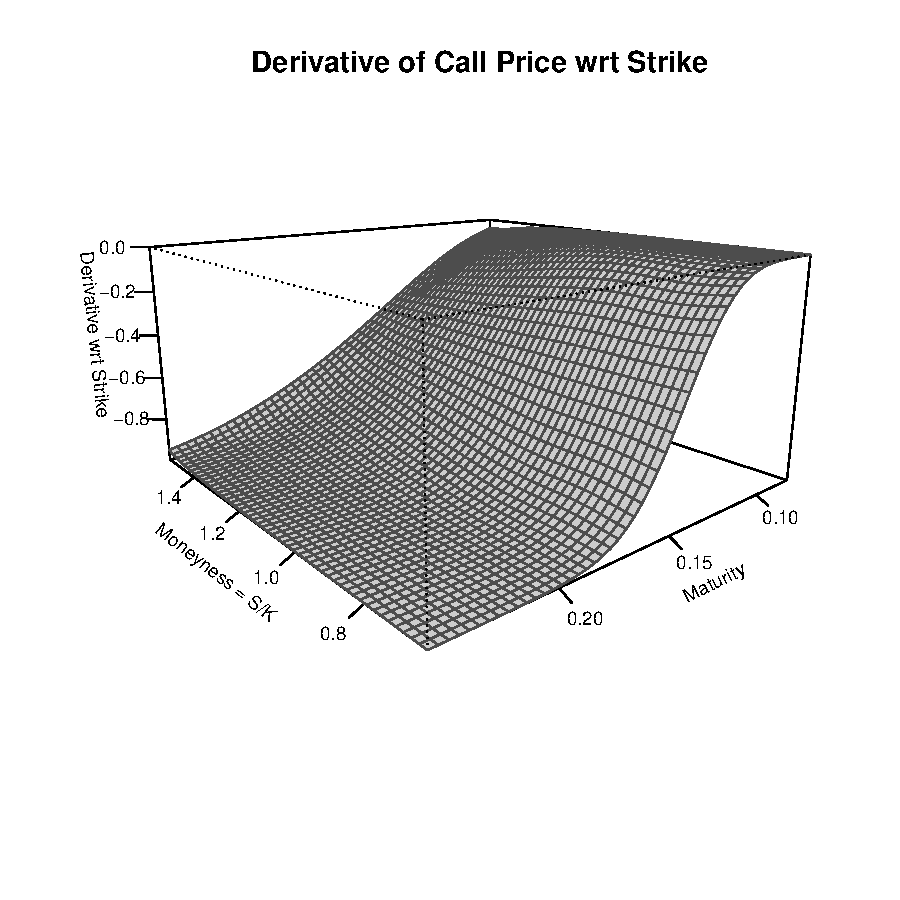
\includegraphics[scale=0.65]{../plots/q3/call_strike_delta.pdf}
 	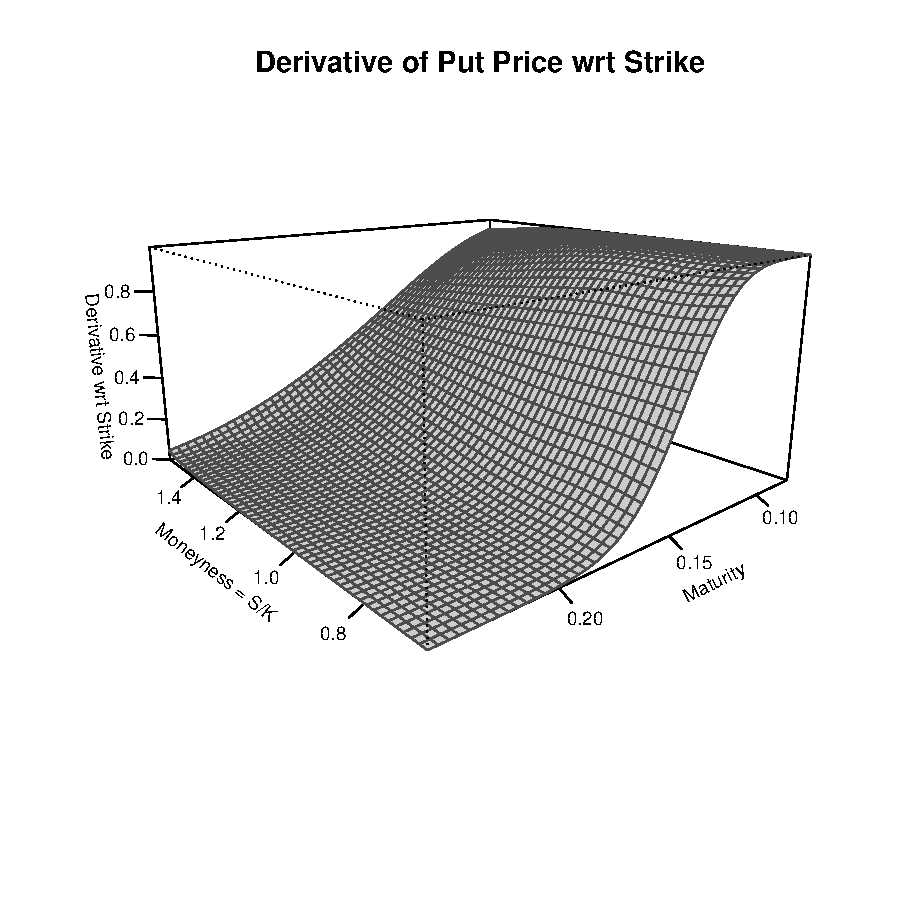
\includegraphics[scale=0.65]{../plots/q3/put_strike_delta.pdf}
\caption{Computed values for (top) $\frac{\partial C}{\partial K}$ and (bottom) $\frac{\partial P}{\partial K}$ given the fitted volatility surface for $h_1 = 0.05, h_2 = 0.05$, with the domain of the fitted surface being the min/max of the observed data.}
\label{fig:strike_delta}
\end{figure}

\begin{figure}[H]
	\centering
 	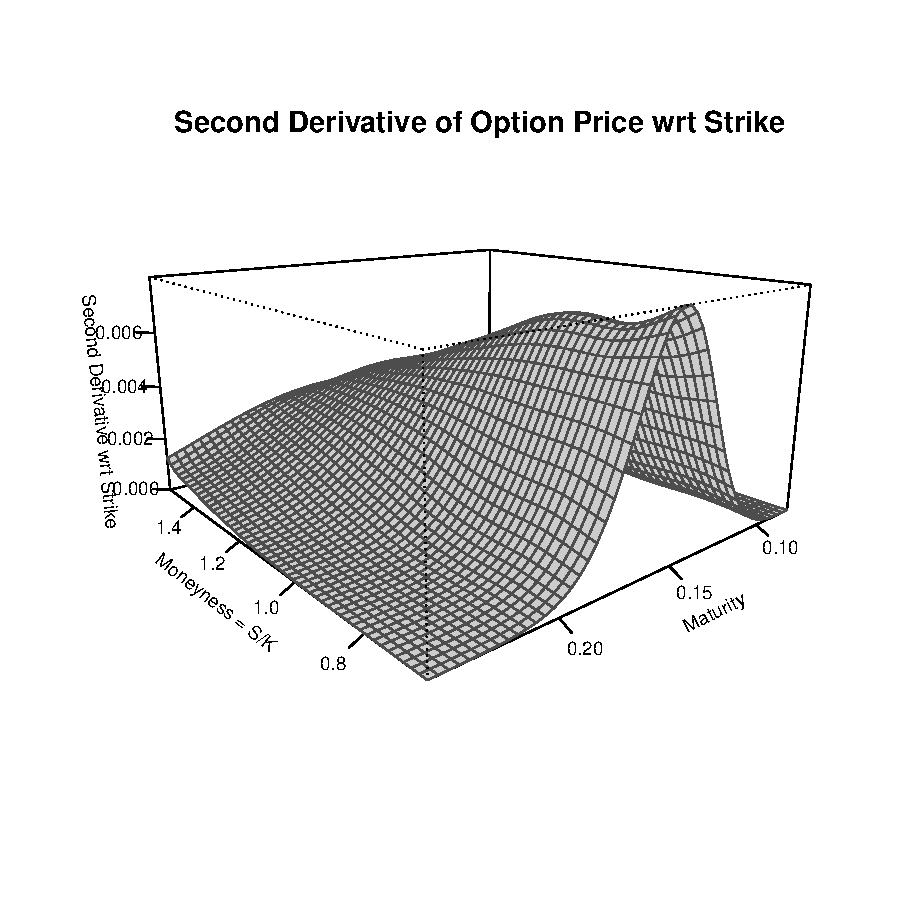
\includegraphics[scale=0.65]{../plots/q3/strike_gamma.pdf}
\caption{Computed values for $\frac{\partial C}{\partial K} = \frac{\partial P}{\partial K}$ given the fitted volatility surface for $h_1 = 0.05, h_2 = 0.05$, with the domain of the fitted surface being the min/max of the observed data.}
\label{fig:strike_gamma}
\end{figure}

\indent Using this fitted surface ($h_1 = 0.05, h_2 = 0.05$, with the min/max of each dimension corresponding to the min/max of the observed data) we see that our volatility estimates do not predict call/put spread arbitrage or butterfly arbitrage opportunities, satisfying the requirements presented above. We are pleased and move on to discussing calendar spread arbitrage. We find that

\begin{align*}
	\frac{\partial C}{\partial T} &= \frac{\partial}{\partial T}\bigg(\Phi(d_1)S - \Phi(d_2)Ke^{-rT} \bigg) \\
	&= \phi(d_1)\frac{\partial d_1}{\partial T}S - \phi(d_2)\frac{\partial d_2}{\partial T}Ke^{-rT} + \Phi(d_2)Kre^{-rT} \quad \text{but} \\
	\frac{\partial d_2}{\partial T} &= \frac{\partial d_1}{\partial T} - \frac{\sigma}{2\sqrt{T}} \quad \text{so} \\
	\frac{\partial C}{\partial T} &= \phi(d_1)\frac{\partial d_1}{\partial T}S - \phi(d_2)\frac{\partial d_1}{\partial T}Ke^{-rT} + \frac{\phi(d_2)Ke^{-rT}\sigma}{2\sqrt{T}} + \Phi(d_2)Kre^{-rT} \\
	&= \frac{\partial d_1}{\partial T}\bigg(\phi(d_1)S - \phi(d_2)Ke^{-rT}\bigg) + \frac{\phi(d_2)Ke^{-rT}\sigma}{2\sqrt{T}} + \Phi(d_2)Kre^{-rT} 
\end{align*}

but we have already shown that $\phi(d_1)S - \phi(d_2)Ke^{-rT} = 0$, so
\begin{align*}
	\frac{\partial C}{\partial T} &= \frac{\phi(d_2)Ke^{-rT}\sigma}{2\sqrt{T}} + \Phi(d_2)Kre^{-rT} \\
	&= Ke^{-rT}\bigg( r\Phi(d_2) + \frac{\sigma\phi(d_2)}{2\sqrt{T}} \bigg)
\end{align*}

and from Put-Call parity we have
\begin{align*}
	C &= P + S - Ke^{-rT} \\
	\implies Ke^{-rT}\bigg( r\Phi(d_2) + \frac{\sigma\phi(d_2)}{2\sqrt{T}} \bigg) &= \frac{\partial P}{\partial T} + Kre^{-rT} \\
	\implies \frac{\partial P}{\partial T} &= Ke^{-rT}\bigg( r\Phi(d_2) + \frac{\sigma\phi(d_2)}{2\sqrt{T}} \bigg) - Kre^{-rT} \\
	&= Ke^{-rT}\bigg( r\Phi(d_2) + \frac{\sigma\phi(d_2)}{2\sqrt{T}} - r\bigg) \\
	&= Ke^{-rT}\bigg( r\big(1 - \Phi(-d_2)\big) + \frac{\sigma\phi(d_2)}{2\sqrt{T}} - r\bigg) \\
	&= Ke^{-rT}\bigg(- r\Phi(-d_2) + \frac{\sigma\phi(d_2)}{2\sqrt{T}}\bigg)
\end{align*}

Thus, for the final no-arbitrage requirement
\begin{equation*}
	\frac{\partial C}{\partial T} \geq 0, \quad \frac{\partial P}{\partial T} \geq 0
\end{equation*}

we have
\begin{equation*}
	Ke^{-rT}\bigg( r\Phi(d_2) + \frac{\sigma\phi(d_2)}{2\sqrt{T}} \bigg) \geq 0, \quad Ke^{-rT}\bigg(- r\Phi(-d_2) + \frac{\sigma\phi(d_2)}{2\sqrt{T}}\bigg) \geq 0
\end{equation*}

\indent If we implement these sufficiently closed form expressions for $\frac{\partial C}{\partial T}, \frac{\partial P}{\partial T}$ with our volatility surface we see the following figures:

\begin{figure}[H]
	\centering
 	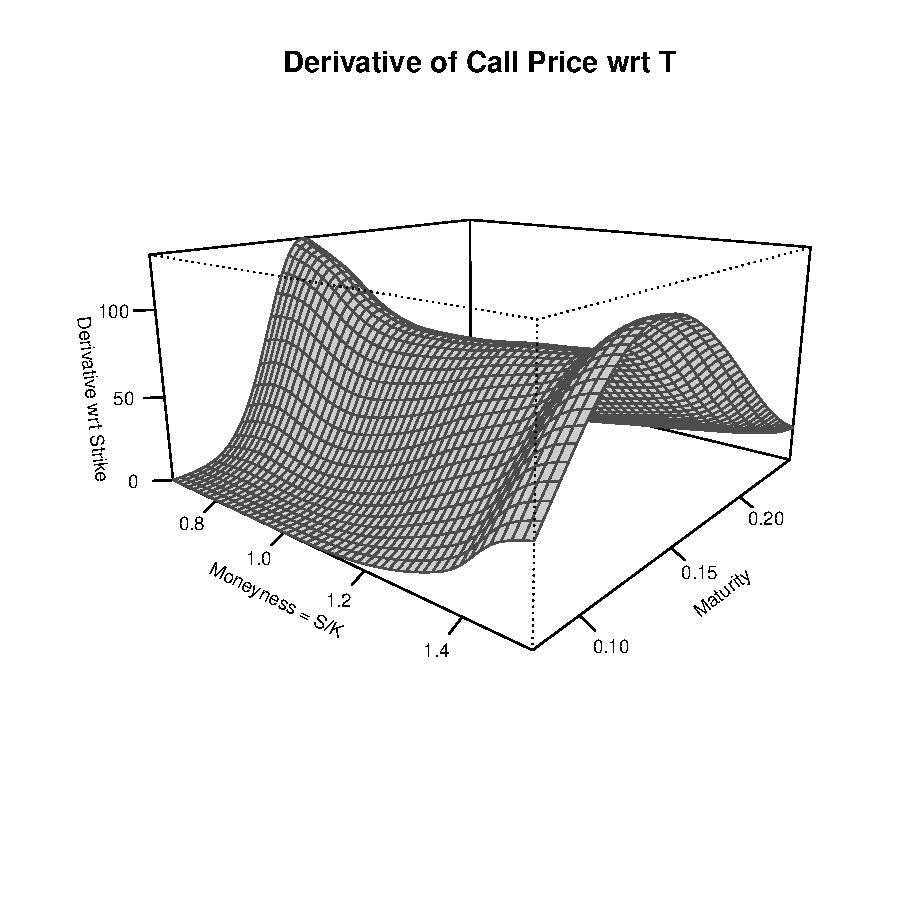
\includegraphics[scale=0.65]{../plots/q3/call_T.pdf}
 	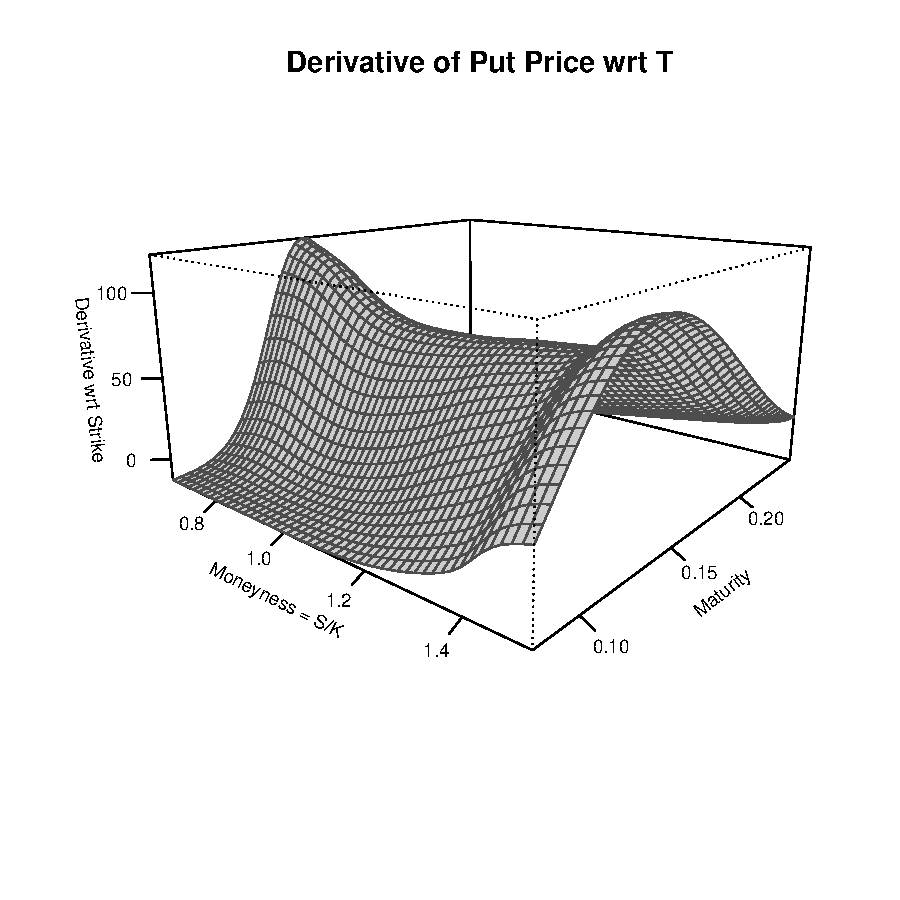
\includegraphics[scale=0.65]{../plots/q3/put_T.pdf}
\caption{Computed values for (top) $\frac{\partial C}{\partial T}$ and (bottom) $\frac{\partial P}{\partial T}$ given the fitted volatility surface for $h_1 = 0.05, h_2 = 0.05$, with the domain of the fitted surface being the min/max of the observed data.}
\label{fig:T}
\end{figure}

\indent Notice that using the fitted volatility surface $(h_1 = 0.05, h_2 = 0.05)$ we satisfy the no calendar spread arbitrage requirement for call options, but for put options we observe some negative values for $\frac{\partial P}{\partial T}$ at extremely low moneyness, short maturity options. Manipulating the smoothing parameters doesn't appear to remedy the situation (plots omitted), leaving these extreme cases predicting arbitrage opportunities. Thus, we suspect that the cause of these calendar spread arbitrage predictions is the presence of outliers in this range of our data set.

\section{Question 4: {\normalfont Pricing a Vanilla Option Based on the Volatility Surface}}

\indent With fixed maturity $T = 60/365$ we wish to price a European call option written on AAPL ($S = 502.12, r = 0.0175$) with strike $K = 572.50$ using our fitted surface. This particular surface used $N = 50$ grid points in each dimension. Finding the fitted volatility corresponding to the moneyness and maturity the nearest to the desired moneyness/maturity we get \\

\begin{lstlisting}
	closest_moneyness = 0.88278
	closest_maturity = 0.164719
	sigma_hat = 0.31168
\end{lstlisting}

\indent We note that this is an error of $0.005714$ in moneynes (strike error = $\$3.7060$). Similarly, we have an error in maturity of $0.0003354$ years, approximately 2.94 hours. With this we price the European call option, and corresponding hedge ratio, \\

\begin{lstlisting}
	bs_price = 5.46787
	bs_hedge_ratio = 0.17053
\end{lstlisting} 

\indent As an exercise, we up the number of grid point in our fitted surface to $N = 100$ in each dimension, we get \\

\begin{lstlisting}
	closest_moneyness = 0.88045	
	closest_maturity = 0.163858
	sigma_hat = 0.312129
\end{lstlisting} 

\indent This which corresponds to a moneyness error of $0.00338$ (strike error = $\$2.2007$) and a maturity error of $0.0005256$ years, approximately 4.96 hours. This values give us \\

\begin{lstlisting}
	bs_price = 5.49106
	bs_hedge_ratio = 0.170923
\end{lstlisting} 

which corresponds to a difference in price of approximately 2.3 cents. For fun, we up the steps to $N = 1000$, giving us \\

\begin{lstlisting}
	closest_moneyness = 0.876652	
	closest_maturity = 0.164436
	sigma_hat = 0.31262
	bs_price = 5.51647
	bs_hedge_ratio = 0.171353
\end{lstlisting} 

with errors of $0.0004135$ in moneyness (strike error = $\$0.2700$) and a maturity error of $0.00005244$ years, approximately 27.56 minutes. These values give us a price difference of approximately 2.5 cents from the previous. Certainly these differences are appreciable to a financial institution, and we may recommend the use of some local averaging of the volatility surface to get a price that is as accurate as possible.

\appendix

\newpage
\section{Supplemental Figures}
\begin{figure}[H]
	\centering
 	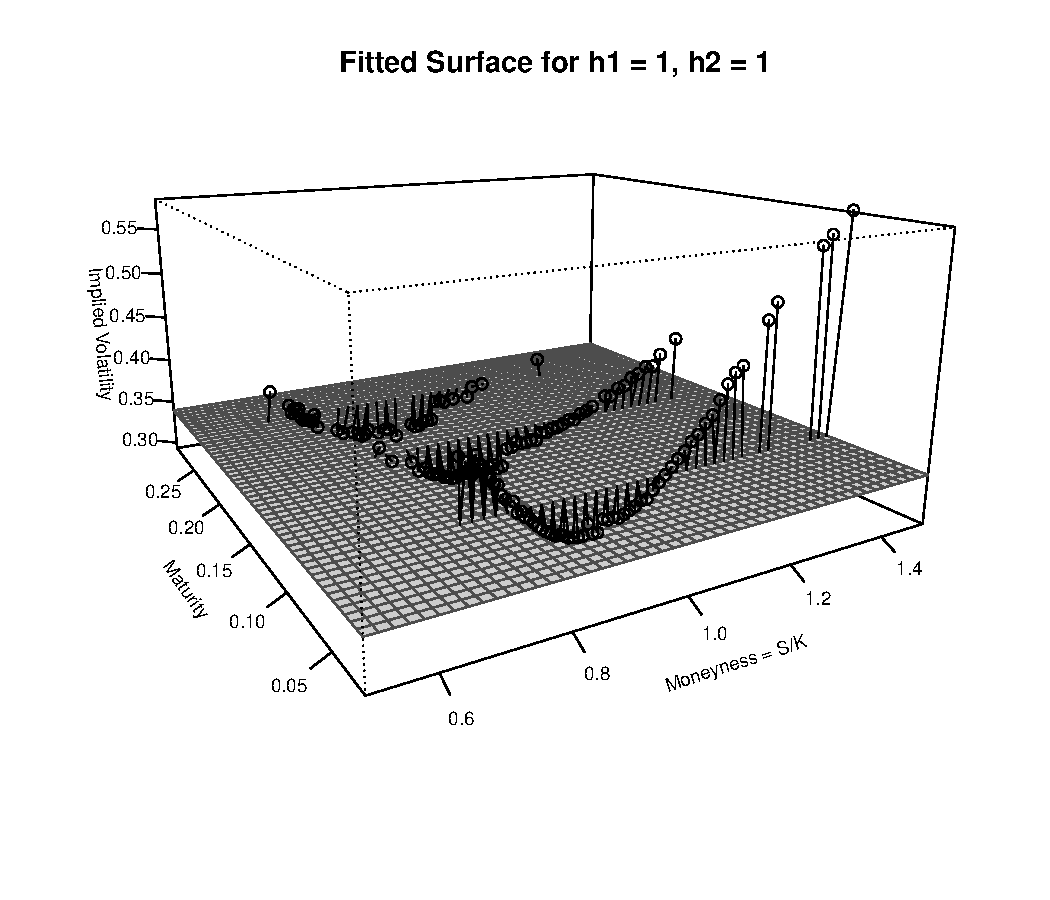
\includegraphics[scale=0.675]{../plots/q2/fitted_2d_1_1.pdf}
 	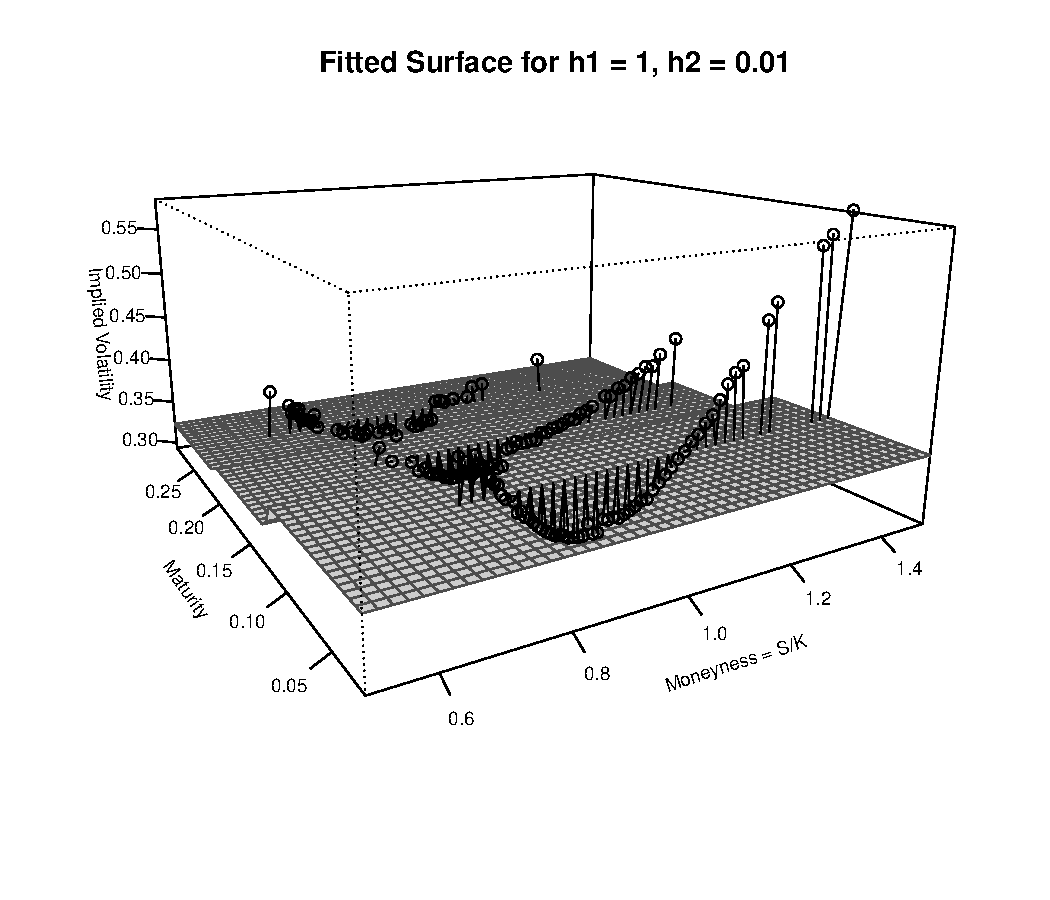
\includegraphics[scale=0.675]{../plots/q2/fitted_2d_1_001.pdf}
\caption{Fitted volatility surface for (top) $h_1 = 1, h_2 = 1$ and (bottom) $h_1 = 1, h_2 = 0.01$.}
\label{fig:fitted_2d_1_1}
\end{figure}

\begin{figure}[H]
	\centering
 	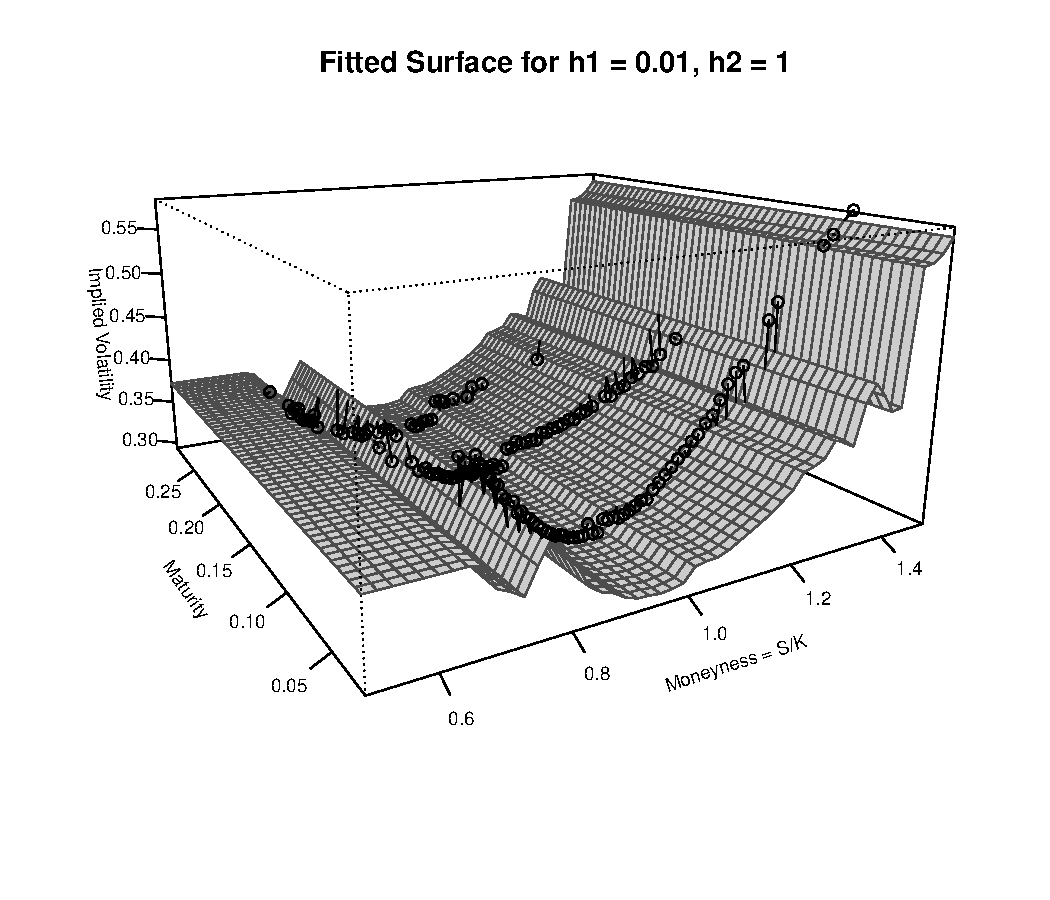
\includegraphics[scale=0.675]{../plots/q2/fitted_2d_001_1.pdf}
	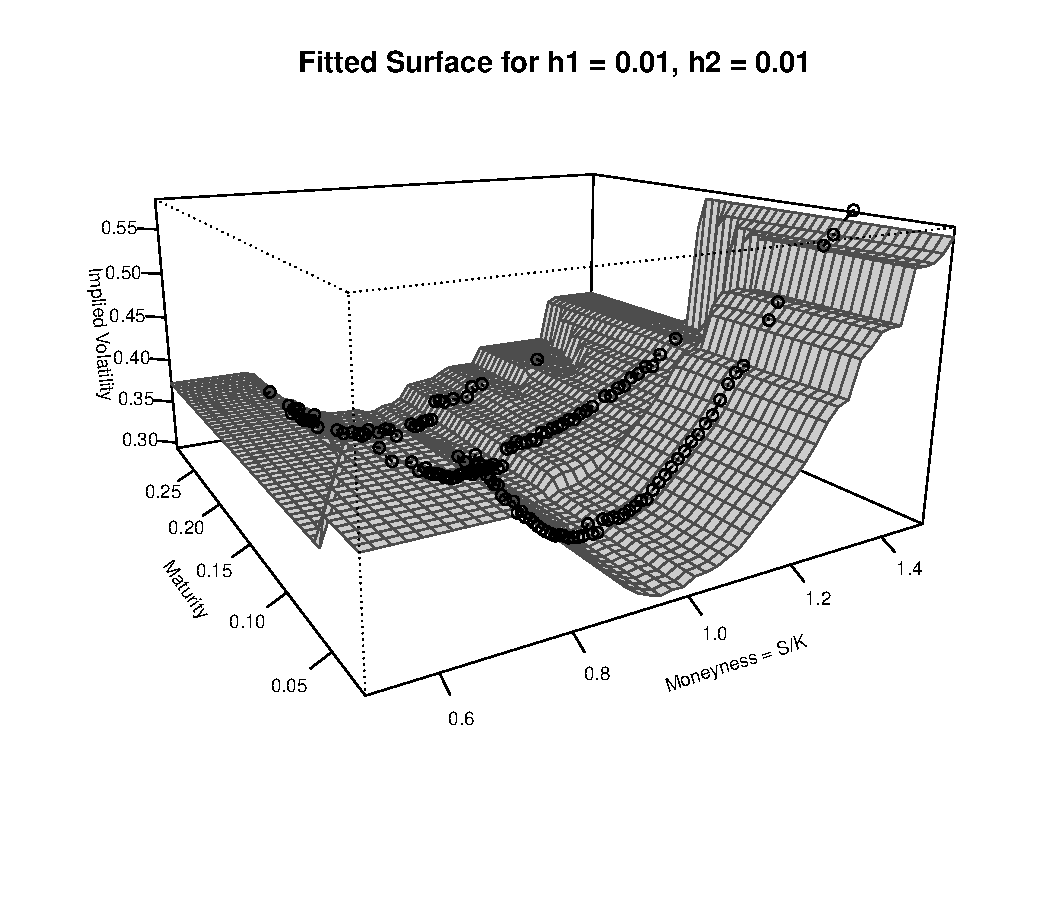
\includegraphics[scale=0.675]{../plots/q2/fitted_2d_001_001.pdf}
\caption{Fitted volatility surface for (top) $h_1 = 0.01, h_2 = 1$ and (bottom) $h_1 = 0.01, h_2 = 0.01$.}
\label{fig:fitted_2d_001_1}
\end{figure}


\newpage
\section{Greeks: Option $\Delta$ and $\nu$}
\footnotesize
The Black-Scholes price of a European call/put option are
\begin{align*}
	C(S,K, t, T, r, \sigma) &= \Phi(d_1)S - \Phi(d_2)Ke^{-r(T - t)} \\
	P(S,K, t, T, r, \sigma) &= \Phi(-d_2)Ke^{-r(T - t)} - \Phi(-d_1)S
\end{align*}

with 
\begin{align*}
	d_1 &= \frac{1}{\sigma\sqrt{T - t}} \bigg[\ln\bigg(\frac{S}{K}\bigg) + \bigg(r + \frac{\sigma^2}{2}\bigg)(T - t) \bigg]\\
	d_2 &= d_1 - \sigma\sqrt{T - t}
\end{align*}

\indent We wish to compute the option Delta, $\Delta_C, \Delta_P$ and option Vega, $\nu_C, \nu_P$. First computing the derivatives for the call price we find
\begin{align*}
	\Delta_C = \frac{\partial C}{\partial S} &= \frac{\partial}{\partial S} \Big( \Phi(d_1)S - \Phi(d_2)Ke^{-r(T - t)} \Big) \\
	&= \Phi'(d_1)\Big(\frac{\partial}{\partial S}d_1\Big)S + \Phi(d_1) - \Phi'(d_2)\Big(\frac{\partial}{\partial S}d_2\Big)Ke^{-r(T - t)} \\
	&= \phi(d_1)\Big(\frac{\partial}{\partial S}d_1\Big)S + \Phi(d_1) - \phi(d_2)\Big(\frac{\partial}{\partial S}d_2\Big)Ke^{-r(T - t)} \\
	\nu_C = \frac{\partial C}{\partial \sigma} &= \frac{\partial}{\partial \sigma} \Big( \Phi(d_1)S - \Phi(d_2)Ke^{-r(T - t)} \Big) \\
	&= \phi(d_1)\Big(\frac{\partial}{\partial \sigma}d_1\Big)S - \phi(d_2)\Big(\frac{\partial}{\partial \sigma}d_2\Big)Ke^{-r(T - t)}
\end{align*}

Computing $\frac{\partial}{\partial S}d_1$ and $\frac{\partial}{\partial S}d_2$,
\begin{align*}
	\frac{\partial}{\partial S}d_1 &= \frac{\partial}{\partial S} \frac{1}{\sigma\sqrt{T - t}} \bigg[\ln\bigg(\frac{S}{K}\bigg) + \bigg(r + \frac{\sigma^2}{2}\bigg)(T - t) \bigg] \\
	&= \frac{1}{S\sigma\sqrt{T - t}} \\
	\frac{\partial}{\partial S}d_2 &= \frac{\partial}{\partial S}(d_1 + \sigma\sqrt{T - t}) = \frac{\partial}{\partial S}d_1 = \frac{1}{S\sigma\sqrt{T - t}} 
\end{align*}

Thus
\begin{align*}
	\Delta_C = \frac{\partial C}{\partial S} &= \phi(d_1)\frac{1}{S\sigma\sqrt{T - t}} S + \Phi(d_1) - \phi(d_2)\frac{1}{S\sigma\sqrt{T - t}} Ke^{-r(T - t)} \\
	&= \Phi(d_1) + \frac{1}{S\sigma\sqrt{T - t}}\Big[S\phi(d_1) - Ke^{-r(T - t)}\phi(d_2) \Big]
\end{align*}

but notice
\begin{align*}
	S\phi(d_1) - Ke^{-r(T - t)}\phi(d_2) = 0 &\iff \frac{S}{K}e^{r(T - t)} = \frac{\phi(d_2)}{\phi(d_1)} \\
	&\iff \ln \frac{S}{K} + r(T - t) = \frac{1}{2}\big(d_1^2 - d_2^2\big) \\
\end{align*}

and
\begin{align*}
	\frac{1}{2}\big(d_1^2 - d_2^2\big) &= \frac{1}{2}(d_1 - d_2)(d_1 + d_2) \\
	&= \frac{1}{2}(d_1 - d_1 + \sigma\sqrt{T - t})(d_1 + d_1 - \sigma\sqrt{T - t}) \\
	&= \frac{\sigma\sqrt{T - t}}{2}(2d_1 - \sigma\sqrt{T - t}) \\
	&= d_1\sigma\sqrt{T - t} - \frac{\sigma^2(T - t)}{2} \\
	&= \frac{1}{\sigma\sqrt{T - t}} \bigg[\ln\bigg(\frac{S}{K}\bigg) + \bigg(r + \frac{\sigma^2}{2}\bigg)(T - t) \bigg] \sigma\sqrt{T - t} - \frac{\sigma^2(T - t)}{2} \\
	&= \ln\bigg(\frac{S}{K}\bigg) + \bigg(r + \frac{\sigma^2}{2}\bigg)(T - t) - \frac{\sigma^2(T - t)}{2} \\
	&= \ln\bigg(\frac{S}{K}\bigg) + r(T - t) 
\end{align*}

Hence
\begin{align*}
	S\phi(d_1) - Ke^{-r(T - t)}\phi(d_2) &= 0 \\
	\implies \Delta_C &= \Phi(d_1) + \frac{1}{S\sigma\sqrt{T - t}}\Big[S\phi(d_1) - Ke^{-r(T - t)}\phi(d_2) \Big] \\
	&= \Phi(d_1)
\end{align*}

For call Vega we note that
\begin{align*}
	\frac{\partial}{\partial \sigma}d_2 &= \frac{\partial}{\partial \sigma}(d_1 - \sigma\sqrt{T - t}) \\
	\implies \frac{\partial}{\partial \sigma}d_1 - \frac{\partial}{\partial \sigma}d_2 &= \sqrt{T - t}
\end{align*}

So
\begin{align*}
	\nu_C = \frac{\partial C}{\partial \sigma} &= \phi(d_1)\Big(\frac{\partial}{\partial \sigma}d_1\Big)S - \phi(d_2)\Big(\frac{\partial}{\partial \sigma}d_2\Big)Ke^{-r(T - t)} \\
	&= \phi(d_1)\Big(\frac{\partial}{\partial \sigma}d_1\Big)S - \phi(d_2)\Big(\frac{\partial}{\partial \sigma}d_2\Big)Ke^{-r(T - t)} - \phi(d_2)\Big(\frac{\partial}{\partial \sigma}d_1\Big)Ke^{-r(T - t)} + \\
	&\hphantom{{}={\phi(d_1)\Big(\frac{\partial}{\partial \sigma}d_1\Big)S -  \phi(d_2)\Big(\frac{\partial}{\partial \sigma}d_2\Big)Ke^{-r(T - t)} - \phi(d_1) }} \phi(d_2)\Big(\frac{\partial}{\partial \sigma}d_1\Big)Ke^{-r(T - t)} \\
	&= \Big(\frac{\partial}{\partial \sigma}d_1\Big)\Big[\phi(d_1)S - \phi(d_2)Ke^{-r(T - t)}\Big] + \phi(d_2)Ke^{-r(T - t)}\Big[-\frac{\partial}{\partial \sigma}d_2 +\frac{\partial}{\partial \sigma}d_1\Big] \\
	&= \Big(\frac{\partial}{\partial \sigma}d_1\Big)\Big[\phi(d_1)S - \phi(d_2)Ke^{-r(T - t)}\Big] + \phi(d_2)Ke^{-r(T - t)}\sigma\sqrt{T - t}
\end{align*}

but
\begin{equation*}
	S\phi(d_1) - Ke^{-r(T - t)}\phi(d_2) = 0 \iff S\phi(d_1) = Ke^{-r(T - t)}\phi(d_2)
\end{equation*}

Hence
\begin{align*}
	\nu_C &= \phi(d_2)Ke^{-r(T - t)}\sigma\sqrt{T - t} \\
	&= S\phi(d_1)\sigma\sqrt{T - t}
\end{align*}

So, for a European call we have
\begin{align*}
	\Delta_C &= \Phi(d_1) \\
	\nu_C &= S\phi(d_1)\sigma\sqrt{T - t}
\end{align*}

Using Put-Call Parity we find the put Delta $\Delta_P$ 
\begin{align*}
	C &= P + S - e^{-r(T - t)}K \\
	\implies \frac{\partial}{\partial S} C &= \frac{\partial}{\partial S} \big(P + S - e^{-r(T - t)}K \big) \\
	\implies \Delta_C &= \Delta_P + 1 \\
	\implies \Delta_P &= \Delta_C - 1 \\
	&= \Phi(d_1) - 1 \\
	&= -\Phi(-d_1)
\end{align*}

and Vega $\nu_P$
\begin{align*}
	\frac{\partial}{\partial \sigma} C &= \frac{\partial}{\partial \sigma} \big(P + S - e^{-r(T - t)}K \big) \\
	\nu_C &= \nu_P
\end{align*}

\newpage
\section{Code}
\subsection{MainQ1.cpp}
\lstinputlisting{../code/q1/MainQ1.cpp}

\subsection{MainQ2.cpp}
\lstinputlisting{../code/q2/MainQ2.cpp}

\subsection{MainQ4.cpp}
\lstinputlisting{../code/q4/MainQ4.cpp}

\subsection{OptionData.h}
\lstinputlisting{../code/q4/OptionData.h}
\subsection{OptionData.cpp}
\lstinputlisting{../code/q4/OptionData.cpp}

\subsection{MathHelp.h}
\lstinputlisting{../code/q4/MathHelp.h}
\subsection{MathHelp.cpp}
\lstinputlisting{../code/q4/MathHelp.cpp}

\subsection{Asset.h}
\lstinputlisting{../code/q4/Asset.h}
\subsection{Asset.cpp}
\lstinputlisting{../code/q4/Asset.cpp}

\subsection{Option.h}
\lstinputlisting{../code/q4/Option.h}
\subsection{Option.cpp}
\lstinputlisting{../code/q4/Option.cpp}

\subsection{CallOption.h}
\lstinputlisting{../code/q4/CallOption.h}
\subsection{CallOption.cpp}
\lstinputlisting{../code/q4/CallOption.cpp}

\subsection{PutOption.h}
\lstinputlisting{../code/q4/PutOption.h}
\subsection{PutOption.cpp}
\lstinputlisting{../code/q4/PutOption.cpp}







\end{document}
























